\documentclass{standalone}
\usepackage{tikz}
\usetikzlibrary{arrows.meta, automata, shapes, positioning}

\begin{document}
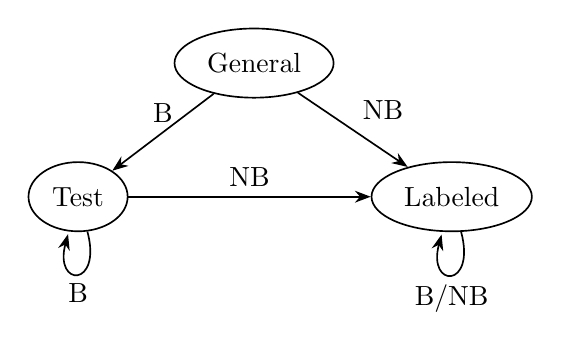
\begin{tikzpicture}[>=Stealth, ->, auto,
    node distance = 1.5cm, semithick]

  \tikzstyle{every state} = [draw, ellipse]

  \node (general) [state] {General};
  \node (test) [state, below left = of general] {Test};
  \node (label) [state, below right = of general] {Labeled};

  \path (general) edge node[above] {B} (test)
		  edge node {NB} (label)
	  (test) edge [loop below] node {B} (test)
		 edge node {NB} (label)
	 (label) edge [loop below] node {B/NB} (label);
\end{tikzpicture}
\end{document}
